\documentclass[17pt]{beamer}
\usecolortheme{seahorse}
\usetheme{default}
\usefonttheme{professionalfonts}
\setbeamertemplate{navigation symbols}{}
\setbeamertemplate{items}[circle]
\setbeamertemplate{blocks}[rounded][shadow=true]

\usepackage[utf8]{inputenc}
\usepackage[T2A]{fontenc}
\usepackage[russian]{babel}
\usepackage{graphicx}
\usepackage{hyperref}
\usepackage{listings}
\usepackage{color}

\hypersetup{unicode=true,
    urlbordercolor=black,
    pdfborderstyle={/S/U/W 1}
}

\lstset{
    extendedchars=\true,
    inputencoding=utf8,
    language=perl,
    showspaces=false,
    showstringspaces=false,
    columns=flexible,
    basicstyle=\small,
    keywordstyle=\color[rgb]{0,0,1},
    commentstyle=\color[rgb]{0.133,0.545,0.133},
    stringstyle=\color[HTML]{AA0000},
}

\newcommand{\otherlink}[2]{
    {\bf #1} \smallskip
    {\small \url{#2}} \bigskip
}

\title{Построение PSGI-совместимых Web-framework'ов}
\author{Сергей Засенко (und3f)}
\date{1 октября 2011 г.}

\begin{document}

\begin{frame}{Black Perl 2011}
\titlepage
\end{frame}

\begin{frame}{Преимущества}

\begin{itemize}
    \item Свобода выбора архитектуры приложения.

% use Moose or don't use Moose.
% one-line controllers
% MVC or not

    \item Возможность простроения асинхронного приложения на базе любой
событийной машины.

% AnyEvent, Coro, POE с возможностью использования всех модулей написанных для
% этих систем

    \item Выбор зависимостей системы.
\end{itemize}
\end{frame}

\begin{frame}{Составляющие веб-фреймворка}

\centering
    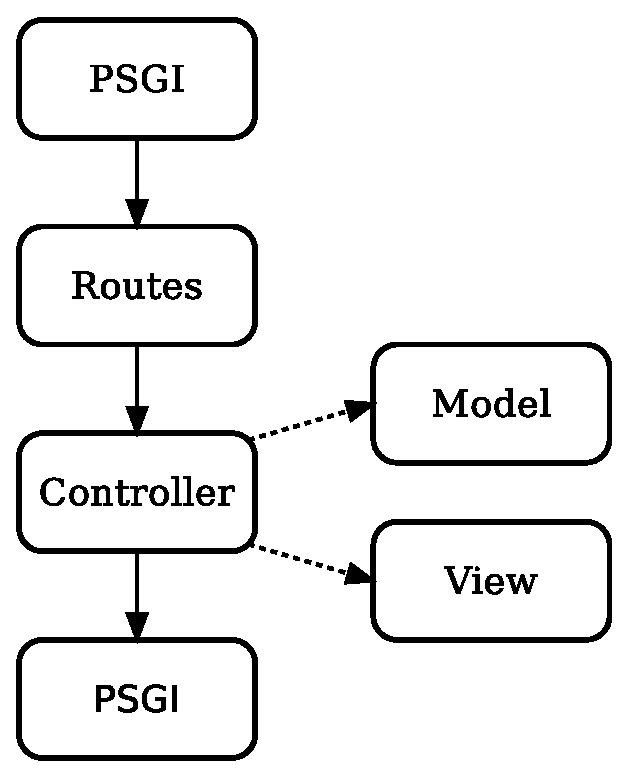
\includegraphics[height=0.8\textheight]{mvc-scheme}

\end{frame}

\begin{frame}{Составляющие веб-фреймворка}

{\bf Routes} --- разбор адреса запроса.

{\bf Controller} --- контроль входящих данных и реализация реакции с
помощью модели и представления.

{\bf View} --- отображение информации.

{\bf Model} --- данные и методы работы с ними.

\end{frame}

\begin{frame}{Что необходимо выполнить?}
\begin{center}
\huge Соединить готовые компоненты
\end{center}
\end{frame}

\begin{frame}{Модули разбора маршрутов}
\begin{itemize}
    \item HTTP::Router
    \item Path::Dispatcher
    \item Path::Router
    \item Route::Simple
    \item Routes::Tiny
    \item другие.
\end{itemize}
\end{frame}

\begin{frame}{Шаблонизаторы}
\begin{itemize}
    \item HTML::CTPP2
    \item HTML::Template
    \item Template::Toolkit
    \item Text::Caml
    \item Text::Xslate
    \item другие.
\end{itemize}
\end{frame}

\begin{frame}{Этапы выполнения}
\begin{enumerate}
\item Разбор адреса запроса и определение обрабатывающего контроллера.
\item Передача управления в соответствующий контроллер.
\item Обработка шаблона с параметрами контроллера.
\end{enumerate}
\end{frame}

\begin{frame}{Реализация}
\begin{center}
    {\huge Hello, {\bf Plack}!}
\end{center}
\end{frame}

\begin{frame}{Инструменты реализации}
\begin{itemize}
    \item Plack
    \item Text::Caml
    \item Routes::Tiny
\end{itemize}
\end{frame}

\begin{frame}[fragile]
\frametitle{Инициализация rout'ов}
\begin{lstlisting}
my $routes = Routes::Tiny->new;

$routes->add_route('/',
    defaults => {action => \&root});

$routes->add_route('/welcome/:name' ,
    defaults => {action => \&welcome});
\end{lstlisting}
\end{frame}

\begin{frame}[fragile]
\frametitle{Разбор URL}
\begin{lstlisting}
sub dispatch {
    my $env = shift;

    my $path = $env->{PATH_INFO};

    if (my $route = $routes->match($path)) {
        my $action = $route->{params}{action};

        $action->($env, $route->{params});
    }
}
\end{lstlisting}
\end{frame}

\begin{frame}[fragile]
\frametitle{View}
\begin{lstlisting}
sub render {
    my ($template, $data) = @_;
    
    my $view = Text::Caml->new;
    
    my $html = $view->render_file($template, $data);

    [200, ['Content-Type', 'text/html'], [$html]];
}
\end{lstlisting}
\end{frame}

\begin{frame}[fragile]
\frametitle{Контроллеры}
\begin{lstlisting}
sub root {
    my ($env, $params) = @_;

    render('root.mt');
}

sub welcome {
    my ($env, $params) = @_;

    render('welcome.mt', $params);
}
\end{lstlisting}
\end{frame}

\begin{frame}[fragile]
\frametitle{Шаблоны}
\lstset{language=html}
\lstinputlisting[title={root.mt}]{sample/root.mt}
\lstinputlisting[title={welcome.mt}]{sample/welcome.mt}
\end{frame}

\begin{frame}[fragile]
\frametitle{Тесты}
\lstset{language=perl}
\begin{lstlisting}
use FindBin '$Bin';
my $app = require "$Bin/../app.psgi";

test_psgi $app, sub {
    my $cb = shift;

    my $res = $cb->(GET '/');
    like $res->content, qr/Hello, Plack!/;

    $res = $cb->(GET '/welcome/Sergey');
    like $res->content, qr/Hello, Sergey./;
}
\end{lstlisting}
\end{frame}

\begin{frame}{Итог}

\begin{itemize}
% Наличие набора готовых компонентов

\item Есть набор готовых компонент для построения собственного web-framework'а.

% Легкое соединение
\item Соединять компоненты легко.
% .....
\item Возможно разработать приложение любой конфигурации.

\item Разрабатывайте!

\end{itemize}
\end{frame}

\begin{frame}{Исходный код}

{\small \url{https://github.com/und3f/black-perl-2011}}

\end{frame}

\begin{frame}{Другие примеры}

\otherlink{JLogger::Web}{https://github.com/und3f/jlogger-web}

\otherlink{Lamework}{https://github.com/vti/lamework}

\otherlink{Web::Simple}{https://metacpan.org/module/Web::Simple}

\end{frame}

\begin{frame}{ }

\centering{\huge Вопросы?}

\end{frame}

\end{document}
